\section{Auswertung}

\subsection{Bestimmung der Zeitkonstante aus dem Entladevorgang}
\label{auswertung:1}

$U$ bezeichnet hierbei die Spannung am Kondensator, die zuvor auch $U_C$ genannt wurde.

\begin{table}
  \centering
  \caption{Messwerte für die Kondensatorspannung in Abhängigkeit der Entladezeit.}
  \label{tab:mess_1}
  \begin{tabular}{S[table-format=1.1] S[table-format=2.1]}
  \toprule
  $t \mathbin{/} \si{\milli\second}$ &
  $U \mathbin{/} \si{\volt}$ \\
  \midrule
  \expandableinput{build/tab/mess_1.tex}
  \bottomrule
  \end{tabular}
\end{table}

Aus \autoref{eqn:entladung} wird
– unter Ausnutzung von $U \propto Q$ –
die Gleichung für eine Regressionsgerade folgendermaßen bestimmt:
\begin{align*}
  U(t) &= U_0 \cdot \exp(-t / RC) \\
  \Leftrightarrow \quad
  \ln(U(t)) &= \underbrace{-\frac{1}{RC}}_a t
  + \underbrace{\ln(U_0)}_b \ .
\end{align*}
Die Parameter werden durch Ausführung der Regression zu
\begin{align*}
  a &= \num{-0.492(10)} \\
  b &= \num{2.686(33)} \\
\end{align*}
bestimmt, woraus die Zeitkonstante
\[ RC = -\frac{1}{a} = \SI{2.03(4)}{\milli\second} \]
folgt.
Messwerte und Regressionsgerade sind in \autoref{fig:1_rc_via_t} dargestellt.

\begin{figure}
    \centering
    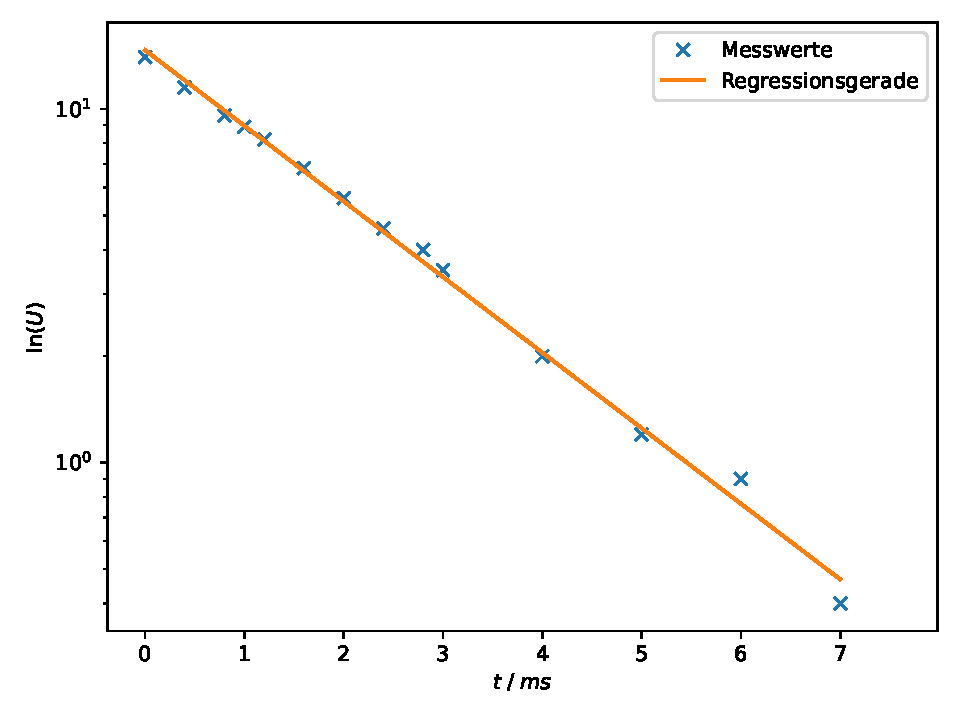
\includegraphics[width=\textwidth]{build/plt/1_rc_via_t.pdf}
    \caption{Messwerte und Regressionsgerade.}
    \label{fig:1_rc_via_t}
\end{figure}

\clearpage
\subsection{Bestimmung der Zeitkonstante aus der Frequenzabhängigkeit}
\label{auswertung:2}

\begin{table}
  \centering
  \caption{Messwerte für die Kondensatorspannung in Abhängigkeit der angelegten Frequenz.}
  \label{tab:mess_2}
  \begin{tabular}{S[table-format=4.0] S[table-format=2.1]}
  \toprule
  $f \mathbin{/} \si{\hertz}$ &
  $U \mathbin{/} \si{\volt}$ \\
  \midrule
  \expandableinput{build/tab/mess_2.tex}
  \bottomrule
  \end{tabular}
\end{table}

Dazu wird ein Fit der in \autoref{eqn:amplitude} erklärten Funktion $A(\omega)$
mittels \texttt{scipy.optimize.curve\_fit} berechnet.
Die bestimmten Parameter lauten
\begin{align*}
  %sollten wir das überhaupt mit fitten? ↓
  U_0 &= \SI{15}{\volt} \\
  RC &= \SI{2.103(18)}{\milli\second} \ .
\end{align*}

In \autoref{fig:2_rc_via_freq} sind Messwerte und Fit dargestellt.

\begin{figure}
    \centering
    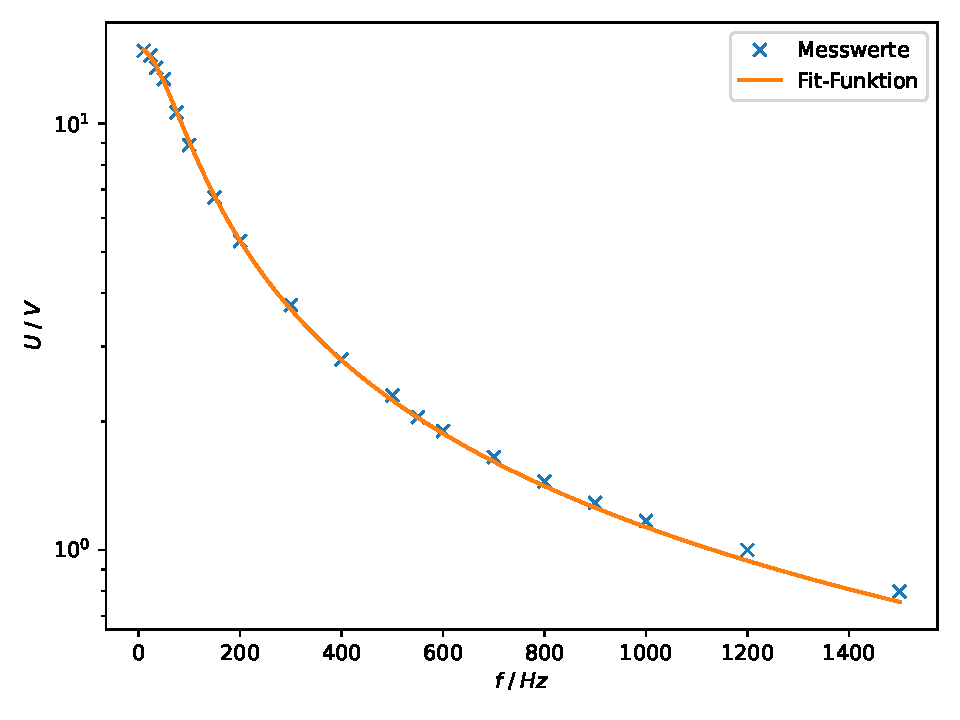
\includegraphics[width=\textwidth]{build/plt/2_rc_via_freq.pdf}
    \caption{Messwerte und Fit-Funktion.}
    \label{fig:2_rc_via_freq}
\end{figure}

\clearpage
\subsection{Bestimmung der Zeitkonstante aus der frequenzabhängigen Phasenverschiebung}
\label{auswertung:3}

Wie zuvor beschrieben wurde,
tritt mit steigender Frequenz zunehmend eine Phasenverschiebung zwischen Kondensatorspannung und Gegenspannung auf.
Auch aus diesem Phänomen lässt sich $RC$ berechnen.
Dazu wird ein Fit für \autoref{eqn:phasenverschiebung} berechnet.
Hier ergibt sich
\[ RC = \SI{11.0(7)}{\milli\second} \ . \]
Aufgrund der großen Abweichung von den zuvor berechneten $RC$ ist in \autoref{fig:3_rc_via_phi}
zum Vergleich auch die erwartete Kurve für diese eingezeichnet.
Dabei wurde die dazwischen liegende Fläche gefüllt.

\autoref{fig:3_polar} zeigt schließlich,
in welchem Verhältnis die Relativamplitude zu der Phase $\varphi$ steht.
Es wurde mit dem gerade bestimmten $RC = \SI{11.0(7)}{\milli\second}$ gerechnet.

\begin{table}
  \centering
  \caption{Messwerte für die Phasenverschiebung
  sowie die daraus berechneten $\frac{1}{f}$ und $\varphi$
  in Abhängigkeit der angelegten Frequenz.}
  \label{tab:3}
  \begin{tabular}{S[table-format=4.0] S[table-format=1.2] S[table-format=2.2] S[table-format=2.2] S[table-format=1.2]}
    \toprule
    $f \mathbin{/} \si{\hertz}$ &
    $a \mathbin{/} \si{\milli\second}$ &
    $b \mathbin{/} \si{\milli\second}$ &
    $\frac{1}{f} \mathbin{/} \si{\milli\second}$ &
    $\varphi \mathbin{/} \si{\radian}$ \\
    \midrule
    \expandableinput{build/tab/3.tex}
    \bottomrule
  \end{tabular}
\end{table}

\begin{figure}
    \centering
    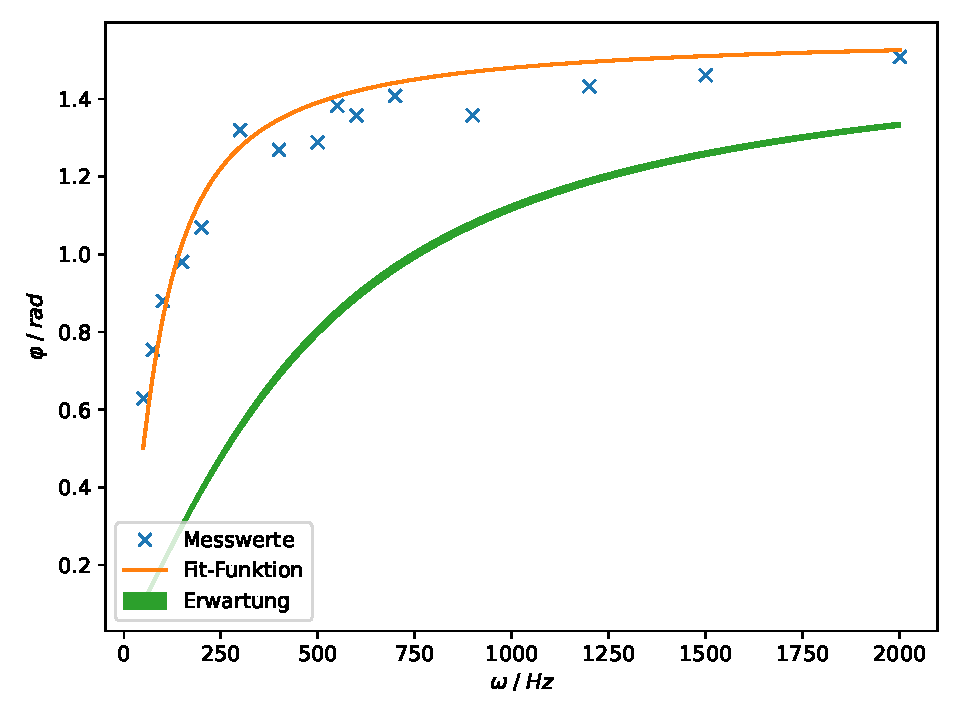
\includegraphics[width=\textwidth]{build/plt/3_rc_via_phi.pdf}
    \caption{Phasenverschiebung in Abhängigkeit der Frequenz.}
    \label{fig:3_rc_via_phi}
\end{figure}

\begin{figure}
    \centering
    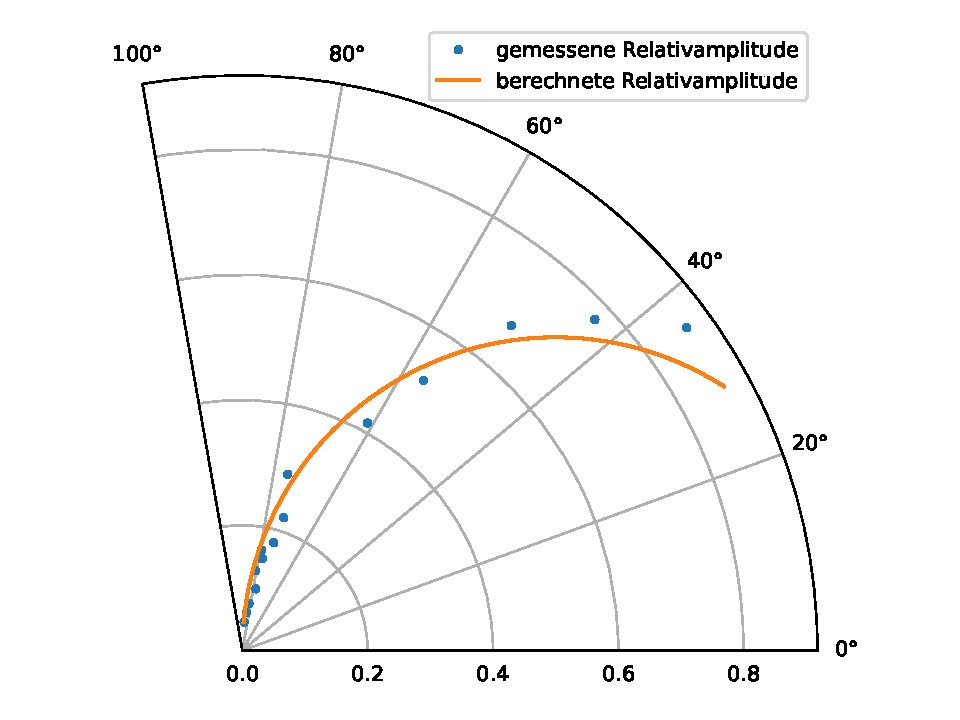
\includegraphics[width=\textwidth]{build/plt/3_polar.pdf}
    \caption{Polar-Plot der gemessenen und berechneten Relativamplituden.}
    \label{fig:3_polar}
\end{figure}
